\chapter{编队控制仿真验证及分析}
\label{chap:hardware}
上一章中完整地介绍了编队控制器的设计方法,以及实际应用时的改进;
本章将介绍编队控制器算法的运行环境,之后使用MATLAB/Simulink
等工具对编队控制器进行数学仿真,再结合ROS/Gazebo仿真环境对编队
控制器进行动力学层面上的仿真验证。
\section{ 软件控制逻辑以及软件环境 }
编队控制算法所运行的软件环境是ROS(Robot Operating System, 机器人操作系统)。ROS是一个为机器人开发而设计的
开源类操作系统平台。本质上,ROS是一个运行于实际操作系统上的应用程序,因而与实际的操作系统有着本质的区别,
但是其对于硬件的抽象以及应用层程序之间的通信的支持使其具有
操作系统的一些重要特征。ROS提供的进程间的通讯方式多种多样,针对于不同要求的应用场景
则设计了不同的进程间的通讯方式,例如消息(Message)、服务(Service)和参数(Param)等;
由于ROS开源社区的蓬勃发展,越来越多的第三方库可以供给开发者使用,也使得针对无人机的
应用开发变得十分方便。本次使用的应用程序接口是
ROS下的mavros功能包,
本功能包的作用是:将来自自动驾驶仪的无人机状态数据由mavlink通信协议转换为ROS的进程间的通讯的协议;
将来自编队控制器的姿态驾驶仪内环的期望姿态角以及期望油门值按照mavlink的协议进行编码,从而起到沟通编队控制器以及姿态驾驶仪内环的桥梁作用。
这里涉及到的Mavlink通讯协议,最早由苏黎世联邦理工大学的研究人员开发,是一种十分轻量级的消息传递协议,广泛用于当今的无人机通讯
,以及无人机内部组件以及无人机与地面站之间的通讯。
MAVLink遵循现代的混合发布-订阅和点对点设计模式:数据流作为主题发送/发布,而配置子协议(如任务协议或参数协议)是点对点重传。
MAVlink通讯已经作为一个专用库封装和发布,通讯时只需要调用相应的库函数进行打包以及包解析,无需再自行定义消息传输格式。
自动驾驶仪则使用第\ref{chap:formation_dynamic_equ}章中介绍的PX4开源自驾仪,此处不再赘述。
\section{无人机编队动力学仿真环境}
所谓无人机动力学仿真环境,是在考虑无人机的动力学过程的基础之上搭建的仿真环境,相较于控制器的数学仿真,此种仿真环境考
虑了无人机作为一个实际的被控系统而存在的过渡过程,不确定性以及扰动因素,将更加还原无人机飞行时的实际状态。
本次动力学仿真环境基于Gazebo这一通用的开源仿真环境,除调用物理引擎仿真飞行器6自由度的动力学模型外,还可以产生相应的、添加噪声
污染的传感器数据反馈给下位机自动驾驶仪。
\begin{figure}[H]
    \centering
    \includegraphics[width=0.75\textwidth]{figures/c4/Gazebo.png}
    \caption{Gazebo仿真环境}\label{fig:c4-Gazebo}
\end{figure}

Gazebo仿真环境可看做由世界(World)、模型(Model)、传感器(Sensor)、物理引擎(Physical Engine)以及插件(Plugin)等模块
组成:世界(World)包含了仿真所使用的全部组件,例如模型(Model)、传感器(Sensor)、灯光(Light)等;模型(Model)的是构成
构成世界的组成部分,可以多次复用。传感器(Sensor)是一类特殊的模型,可以产生带有噪声的传感器数据信息。物理引擎(Physical Engine)
是驱动模型运动的组件,对应的物理库为基本仿真组件提供了一个简单和通用的界面,包括刚体、碰撞形状和表示关节约束的关节。
这个接口集成了四个开源物理引擎。

Gazebo在仿真时,首先加载世界,包括其中的各种参数如重力场定义、灯光等,以及定义了飞机4通道操纵机构飞机模型;
之后,各类插件,例如空气动力学插件、传感器插件以及环境插件等调用物理引擎接口,产生诸如无人机刚体运动学,传感器噪声
、大气环境等相关等相关仿真过程量。至此,通过Gazebo的GUI可以在可视化界面上得到无人机的运动图像。通过PX4官方给出的仿真工具,
可将在Gazebo中运行的固定翼无人机传感器的测量原始信息编码成MAVlink消息格式,反之亦然,之后,再通过TCP4560端口与PX4自驾仪进行通讯,即
Gazebo中的相应控制舵面运动的插件接受来自PX4的控制器信息,再将仿真的传感器数据进行打包和发送,从而构成了仿真环境。

总而言之,Gazebo考虑了无人机详细的动力学方程,只是在空气动力和力矩的产生方面,使用了简单的工程化的计算方法,使用速度、翼面积、
升阻系数等来计算无人机所受的力和力矩,无法模拟细致入微的空气动力学特性;因而不能使用Gazebo环境进行诸如油耗测试等涉及空气动力学
影响的仿真实验。但是,在编队控制器设计与仿真阶段,利用Gazebo仿真不失为一种有效的验证算法的手段。

另外,仿真之中的飞机的动力学模型由Gazebo仿真环境给出,可自定义飞机的质量,推力等参数;仿真之中的传感器数据由Gazebo产生,由PX4读取,作为
真实环境之中的传感器数据的仿真。上述参量均可以按照本次无人机平台做出相应的修改。

基于ROS的编队控制程序同时运行,通过mavros等程序API进行数据交互,完成动力学仿真。
相应的仿真程序之间的逻辑关系如下图所示:
\begin{figure}[H]
    \centering
    \includegraphics[width=0.75\textwidth]{figures/c4/px4_sitl_overview.png}
    \caption{编队控制仿真逻辑}\label{fig:px4_sitl_overview}
\end{figure}
在启动双机仿真时,启动脚本会加载两个无人机模型,并将与其相关的ROS消息用形如“UAV0、UAV1”等编号形式进行区分。
%TODO:需要添加Gazebo的动力学模型是如何载入进来的。
\section{基于MATLAB/Simulink的双机编队数学仿真}
本节数学仿真只验证编队控制器的控制性能以及控制逻辑的正确性,因而在仿真之前,做如下假设:
\begin{enumerate}
\item 无人机自动驾驶仪内环仅为一个具有时间常数$\tau$一阶惯性环节。
\item 无人机的姿态动力学没有过渡过程,即姿态动力学方程由相应的稳态方程代替。
\end{enumerate}
另外,按照第\ref{chap:controller_design}章中控制器设计分为水平平面以及竖直平面的原则,本节之中的仿真也是分为两个方面进行的;在任何
在其中任意一个平面内仿真时,都假设另外一个平面已经达到了控制目标,并且处于稳态。

在水平面的仿真中:选取的初始条件均为在地面坐标系NED中定义,其值如下表所示:
\begin{table}[H]
    \centering
    \caption{水平面内数学仿真初始运动学量} \label{tab:matlab_init_cond}
    \begin{tabular*}{0.9\textwidth}{@{\extracolsep{\fill}}c|cccc}
        \toprule
        指标     & 初速度(m/s)   & 初始位置(m)    & 航迹角(°) & 高度(m)  \\
        \midrule
        领机     & (20.0,0.0)  & (-50.0,100.0) & 0.0        & 100.0 \\
        从机     & (10.0,10.0) & (0.0,100.0)  & 45.0       & 0.0   \\
        \bottomrule
    \end{tabular*}
\end{table}
水平面内的编队控制器的参数,包括两个通道的误差混合参数以及增量式PID的参数:
\begin{table}[H]
    \centering
    \caption{水平面内编队控制器参数} \label{tab:matlab_PID_param}
    \begin{tabular*}{0.9\textwidth}{@{\extracolsep{\fill}}c|ccccc}
        \toprule
        参数 & 比例$K_P$     & 积分$K_I$    & 微分$K_D$ & 混合参数1 & 混合参数2  \\
        \midrule
        X & 0.5 & 0.01  & 0.008  & 0.45  & 0.65 \\
        Y & 0.7 & 0.005 & 0.0015 & 0.008 & 0.5 \\
        \bottomrule
    \end{tabular*}
\end{table}

仿真的结果如下三图所示:其中,图\ref{fig:c5-matlab-pos},表示双机编队位置关系,横轴为NED坐标系下的E轴,纵轴为N轴。
图\ref{fig:c5-matlab-vel}以及图\ref{fig:c5-matlab-eta}分别表示双机速度大小以及速度方向的与时间的关系图。由仿真结果可得,
在算法层面上,第\ref{chap:controller_design}所设计的编队控制器在水平平面内可以完成编队控制的任务。
\begin{figure}[H]
    \centering
    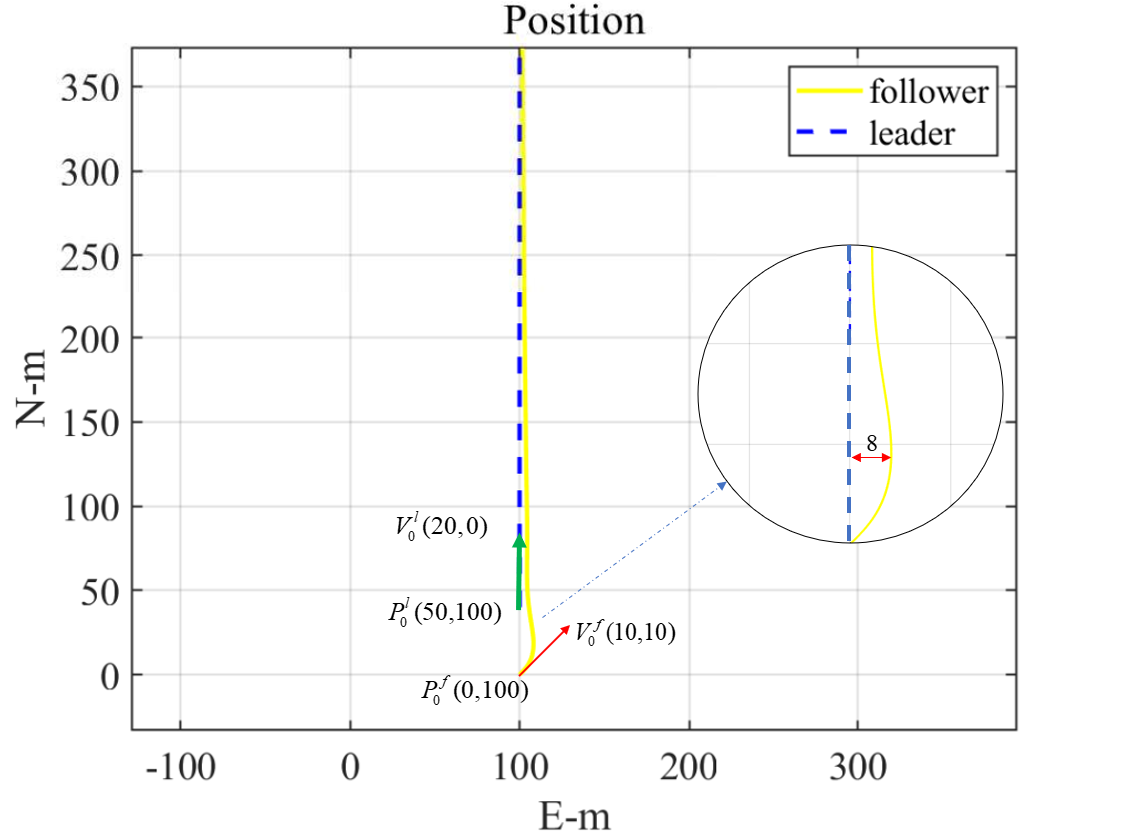
\includegraphics[width=0.85\textwidth]{figures/c5/c5-matlab-pos.png}
    \caption{水平面双机编队位置关系}\label{fig:c5-matlab-pos}
\end{figure}
\begin{figure}[H]
    \centering
    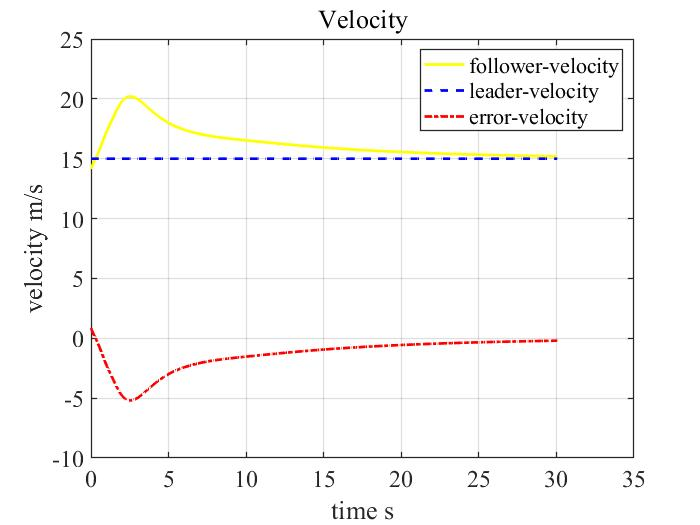
\includegraphics[width=0.85\textwidth]{figures/c5/c5-matlab-vel.jpg}
    \caption{水平面双机速度大小关系}\label{fig:c5-matlab-vel}
\end{figure}
\begin{figure}[H]
    \centering
    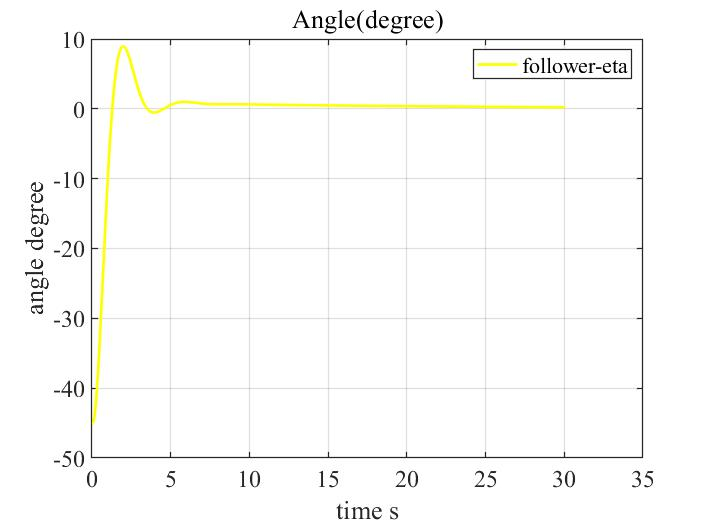
\includegraphics[width=0.85\textwidth]{figures/c5/c5-matlab-eta}
    \caption{水平面双机航迹角关系}\label{fig:c5-matlab-eta}
\end{figure}

竖直平面内,由于控制器的任务是消除高度误差以及追踪来自水平平面控制器的期望速度,控制量将是期望推力$T^{des}$以及期望俯仰角$\theta^{des}$,因而需要引入竖直平面内的无人机动力学模型(参见式\ref{point_dynamaic});按照之前的假设,无人机姿态内环为理想环节,可以用一个时间常数为$\tau_{\theta}$的惯性环节代替之。再结合式\ref{fol_motion_eauation},可以进行竖直平面的相关仿真:
仿真时的领机从机初始运动学量为:
\begin{table}[H]
    \centering
    \caption{竖直面内数学仿真初始运动学量} \label{tab:matlab_vel_cond}
    \begin{tabular*}{0.9\textwidth}{@{\extracolsep{\fill}}c|cc}
        \toprule
        指标 & 初速度(m/s)    & 初始高度(m)\\
        \midrule
        领机 & 20.0  & 10.0\\
        从机 & 10.0 & 100.0\\
        \bottomrule
    \end{tabular*}
\end{table}
竖直内TECS控制器的参数如下表所示:
\begin{table}[H]
    \centering
    \caption{竖直面内TECS控制器参数} \label{tab:matlab_TECS_param}
    \begin{tabular*}{0.9\textwidth}{@{\extracolsep{\fill}}c|cccc}
        \toprule
        TECS参数 & 油门时间常数 & 俯仰角时间常数 & 俯仰角阻尼 & 油门阻尼   \\
        \midrule
        值       & 4.0            & 3.0              & 0.7        & 0.65   \\
        \bottomrule
    \end{tabular*}
\end{table}
\begin{table}[H]
    \centering
    \caption{竖直面内TECS控制器参数(续表)} \label{tab:matlab_TECS_param_app}
    \begin{tabular*}{1.0\textwidth}{@{\extracolsep{\fill}}c|cccc}
        \toprule
        TECS参数 & 积分增益 & 俯仰角-速度比重常数 & 高度误差比例增益 & 速度误差比例增益  \\
        \midrule
        值       & 0.3      & 1.0                   & 0.05             & 0.02     \\
        \bottomrule
    \end{tabular*}
\end{table}

为了方便读图,现在将$NED$坐标系下的$D$轴取反之后并用“$height$”表示,
仿真的结果如下三图所示:
\begin{figure}[H]
    \centering
    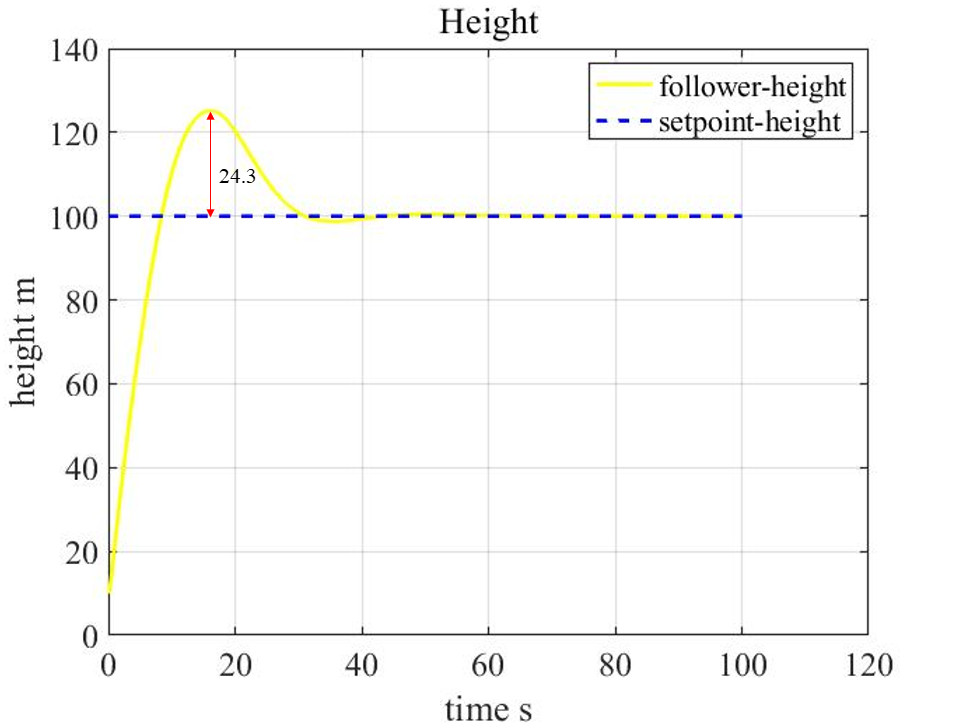
\includegraphics[width=0.85\textwidth]{figures/c5/c5-TECS-height.jpg}
    \caption{竖直平面高度关系}\label{fig:c5-TECS-height}
\end{figure}
\begin{figure}[H]
    \centering
    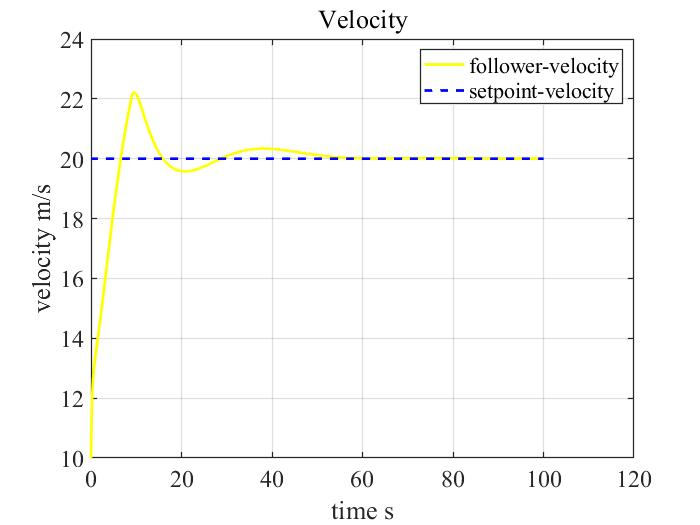
\includegraphics[width=0.85\textwidth]{figures/c5/c5-TECS-vel.jpg}
    \caption{竖直平面速度关系}\label{fig:c5-TECS-vel}
\end{figure}
\begin{figure}[H]
    \centering
    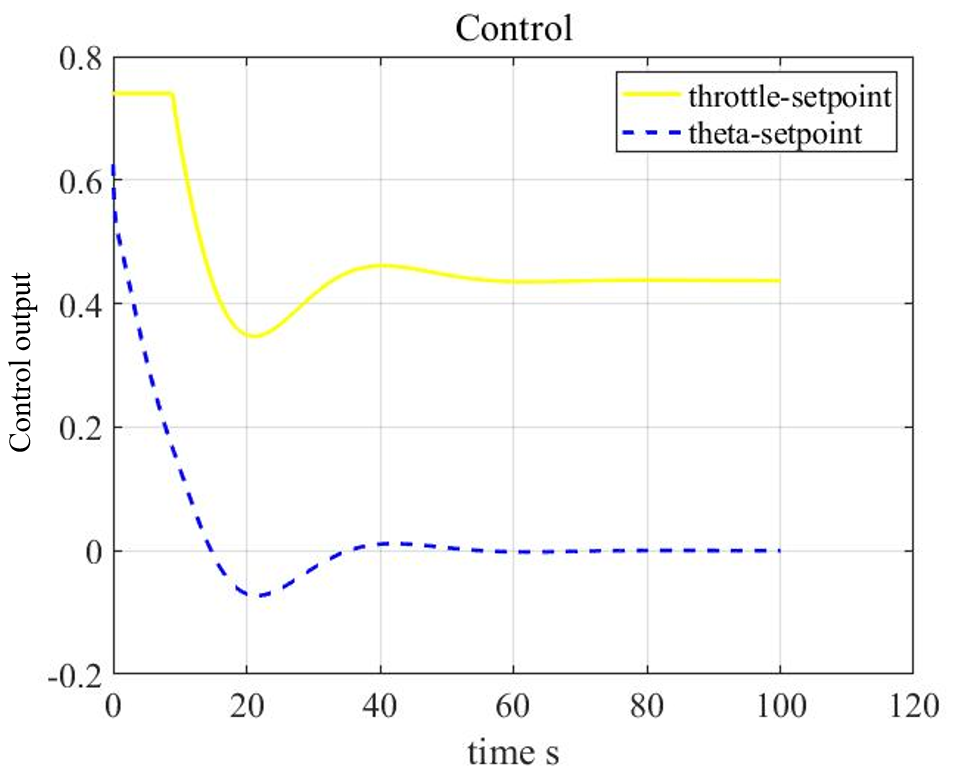
\includegraphics[width=0.80\textwidth]{figures/c5/update/control_output}
    \caption{竖直平面控制量关系}\label{fig:c5-TECS-control}
\end{figure}
由仿真结果可知,本文所设计的TECS控制器可以完成对于期望速度以及期望高度的跟踪,从而达到消除竖直平面内的误差的作用。
\section{基于ROS/Gazebo-PX4的双机编队动力学仿真}
根据第\ref{chap:hardware}章中介绍的ROS-Gazebo仿真环境,进行仿真环境下的双机编队飞行试验。首先利用QGround Control 地面站为领机规划
一条包括起飞以及降落航点在内的一条长直航线。之后先使用地面站将领机1(vehicle 1)
解锁,切换任务模式之后起飞,按照既定航线飞行。等待领机到达第一个
航点之后,再起飞从机2(vehicle 2)
,并切换到外部控制模式,即编队控制的控制逻辑。之后经过一段时间的飞行之后,采集飞行之中的编队误差等数据:最终
编队稳定之后的可视化效果如下:
\begin{figure}[H]
    \centering
    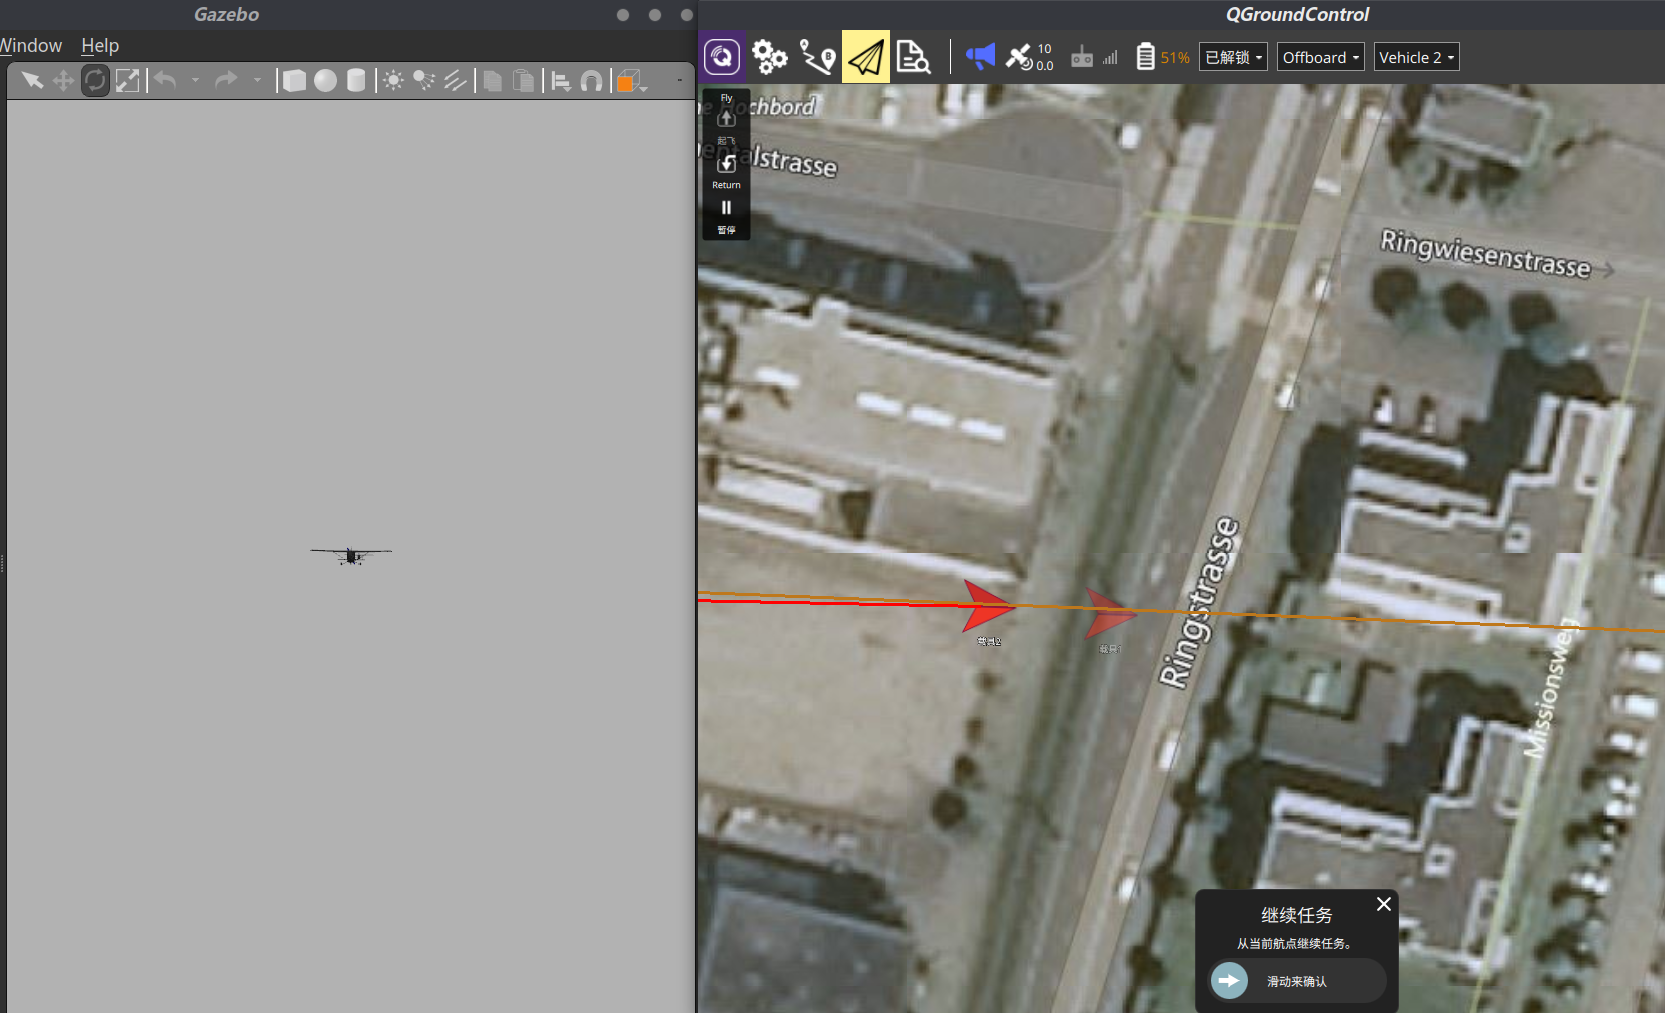
\includegraphics[width=0.85\textwidth]{figures/c5/c5-real-overview}
    \caption{稳定编队之后的编队可视化效果}\label{c5-real-overview}
\end{figure}
动力学仿真的初始条件如下表所示:
\begin{table}[H]
    \centering
    \caption{Gazebo双机编队动力学仿真初始条件} \label{tab:real_init_cond}
    \begin{tabular*}{0.9\textwidth}{@{\extracolsep{\fill}}c|cccc}
        \toprule
        指标     & 初速度(m)     & 初始位置(m)  & 航迹角(°) & 高度(m)  \\
        \midrule
        领机     & (0.0,0.0)    & (0.0,80.0) & 90    & 100.0 \\
        从机     & (0.0,15.0) & (0.0,0.0)   & 90    & 0.0   \\
        \bottomrule
    \end{tabular*}
\end{table}
动力学仿真过程中的编队控制器的控制器参数如下表所示:
\begin{table}[H]
    \centering
    \caption{水平面内控制器参数} \label{tab:real_PID_param}
    \begin{tabular*}{0.9\textwidth}{@{\extracolsep{\fill}}c|ccccc}
        \toprule
        参数 & 比例$K_P$     & 积分$K_I$    & 微分$K_D$ & 混合参数1 & 混合参数2  \\
        \midrule
        X & 0.3 & 0.01  & 0.008  & 0.4   & 0.65 \\
        Y & 0.4 & 0.005 & 0.0015 & 0.005 & 0.4 \\
        \bottomrule
    \end{tabular*}
\end{table}
TECS控制器的参数如下表所示:
\begin{table}[H]
    \centering
    \caption{竖直面内TECS控制器参数} \label{tab:real_TECS_param}
    \begin{tabular*}{0.9\textwidth}{@{\extracolsep{\fill}}c|cccc}
        \toprule
        TECS参数 & 油门时间常数 & 俯仰角时间常数 & 俯仰角阻尼 & 油门阻尼   \\
        \midrule
        值       & 8            & 5              & 0.3        & 0.5   \\
        \bottomrule
    \end{tabular*}
\end{table}
\begin{table}[H]
    \centering
    \caption{竖直面内TECS控制器参数(续表)} \label{tab:real_TECS_param_app}
    \begin{tabular*}{1.0\textwidth}{@{\extracolsep{\fill}}c|cccc}
        \toprule
        TECS参数 & 积分增益 & 俯仰角-速度比重常数 & 高度误差比例增益 & 速度误差比例增益  \\
        \midrule
        值      & 0.1  & 1          & 0.05     & 0.02     \\
        \bottomrule
    \end{tabular*}
\end{table}
在仿真过程中,利用ROS提供的rosbag等数据记录工具,可以进行仿真之中的数据记录与处理:
图\ref{c5-real-pos_err_x}-图\ref{c5-real-pos_err_z}分别代表了双机编队位置误差投影
在从机坐标系$O_kx_ky_kz_k$中的分量随时间的变化关系;图\ref{c5-real-eta_err}代表从
机与领机的速度方向误差随时间变化关系;图\ref{c5-real-vel_err}代表从机与领机的速度大小误差随时间的变化关系。
\begin{figure}[H]
    \centering
    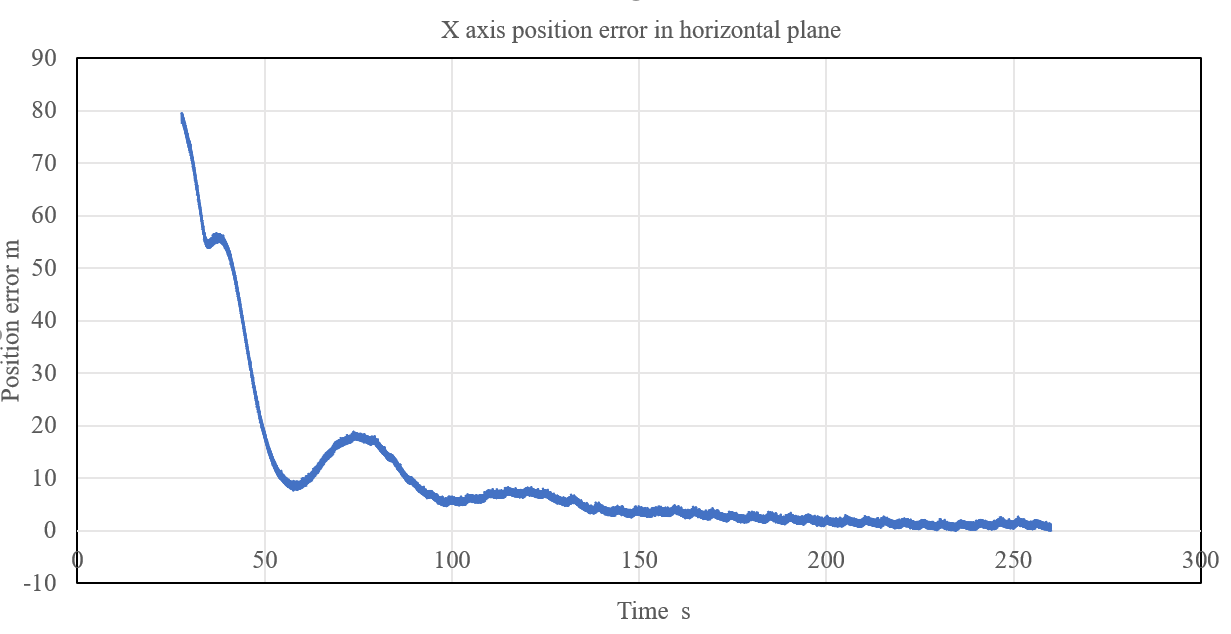
\includegraphics[width=0.85\textwidth]{figures/c5/update/pos_x}
    \caption{X通道位置误差}\label{c5-real-pos_err_x}
\end{figure}
\begin{figure}[H]
    \centering
    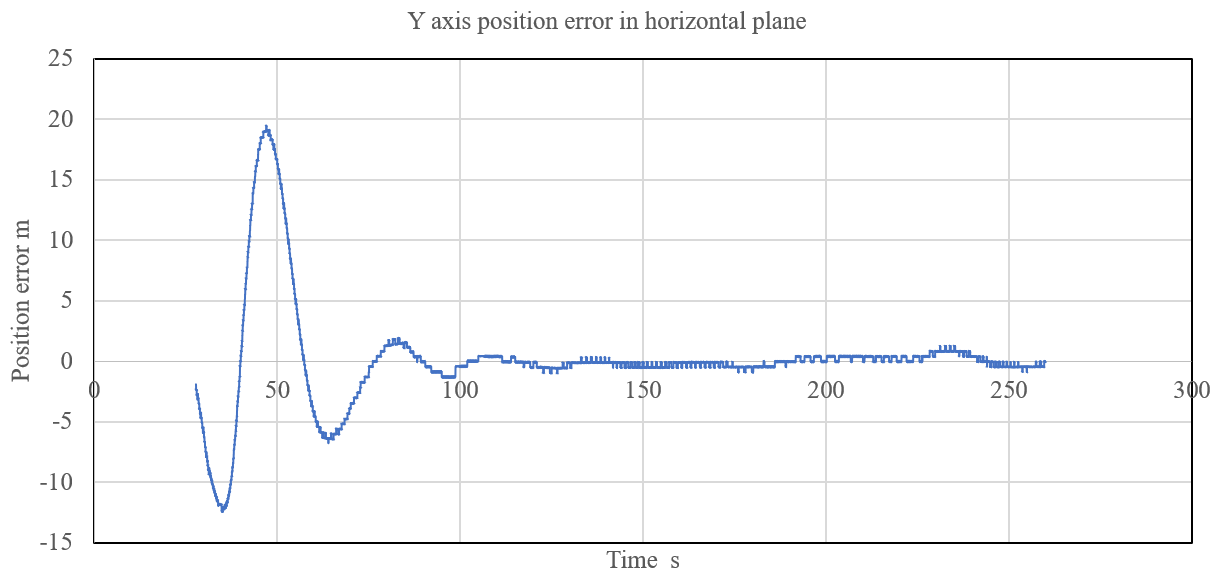
\includegraphics[width=0.85\textwidth]{figures/c5/update/pos_y}
    \caption{Y通道位置误差}\label{c5-real-pos_err_y}
\end{figure}
\begin{figure}[H]
    \centering
    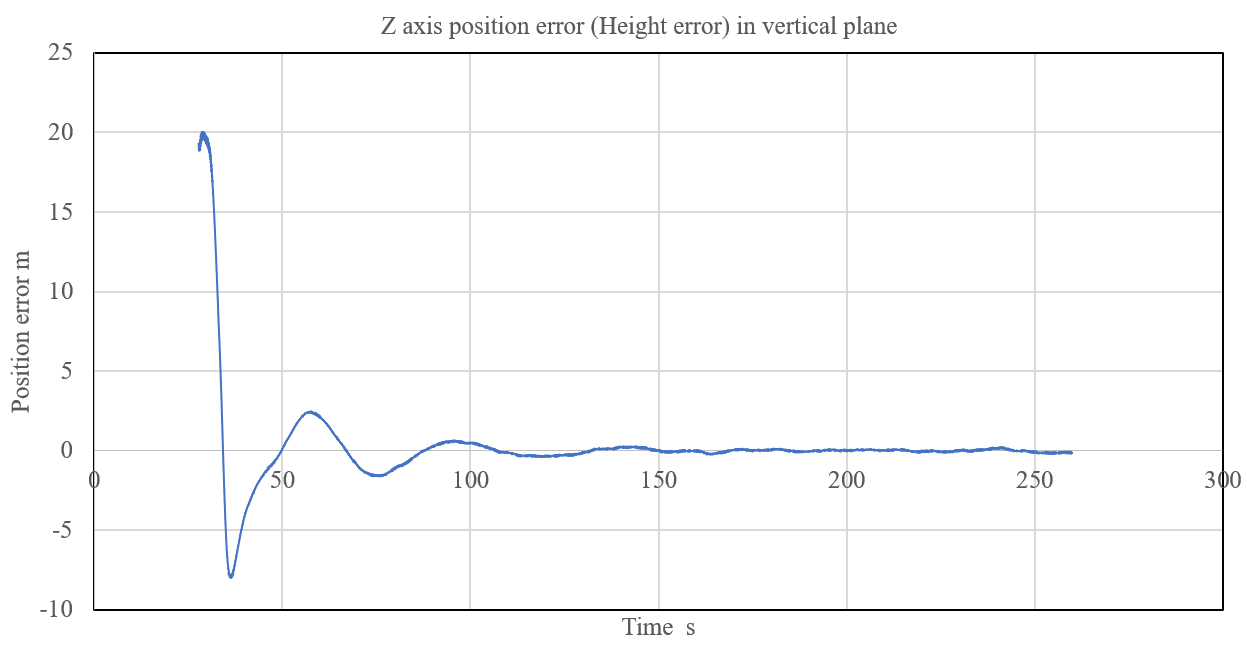
\includegraphics[width=0.85\textwidth]{figures/c5/update/pos_z}
    \caption{Z通道位置误差}\label{c5-real-pos_err_z}
\end{figure}
\begin{figure}[H]
    \centering
    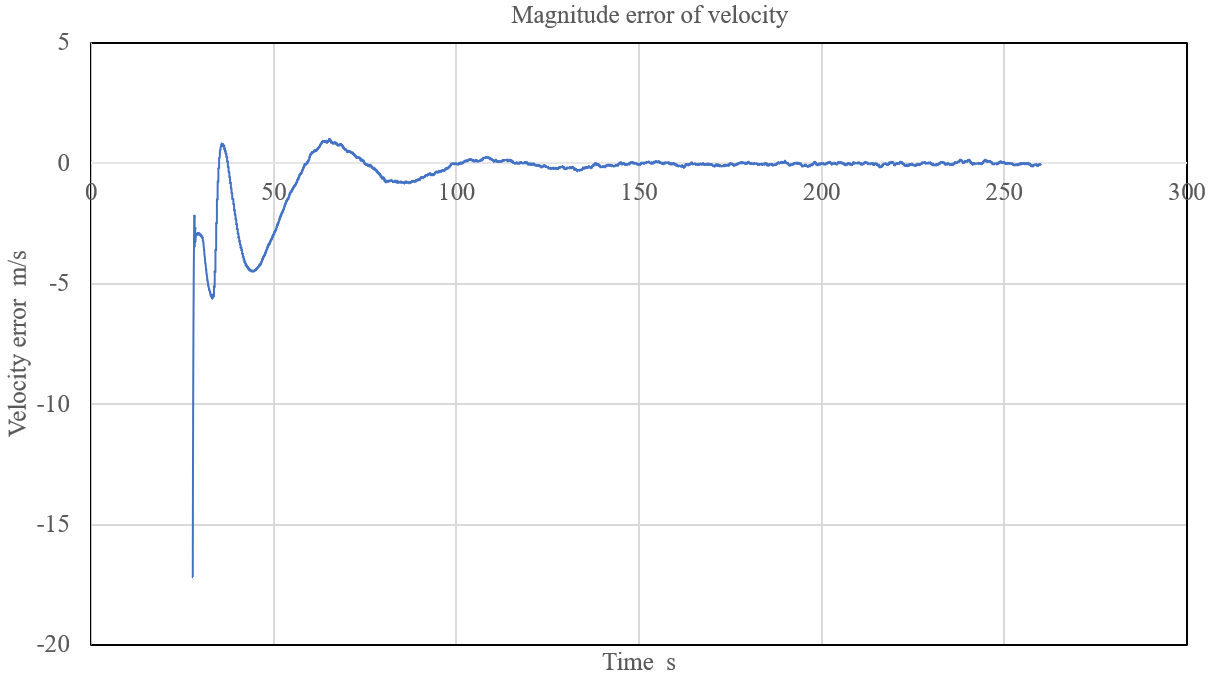
\includegraphics[width=0.85\textwidth]{figures/c5/update/vel}
    \caption{领机从机速度大小误差}\label{c5-real-vel_err}
\end{figure}
\begin{figure}[H]
    \centering
    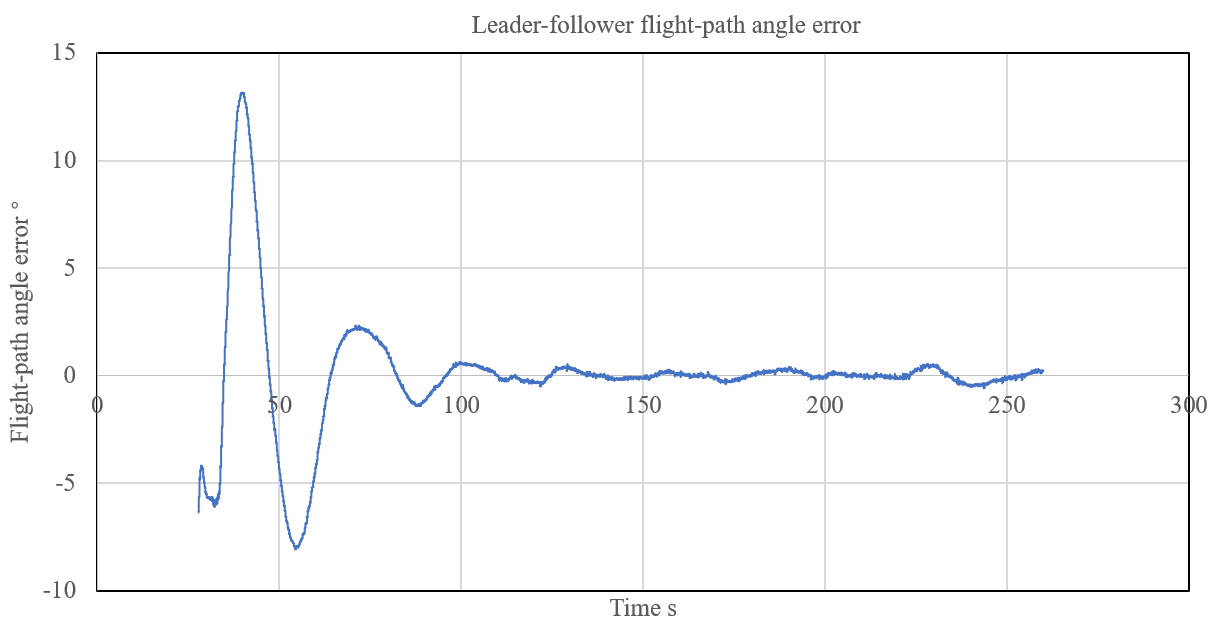
\includegraphics[width=0.85\textwidth]{figures/c5/update/angle}
    \caption{领机从机航迹角误差}\label{c5-real-eta_err}
\end{figure}
需要注意的一点是:此处的位置误差指的是从机的实际位置与编队的期望位置之间的位值误差,而并非与领机的位置误差。
从图\ref{c5-real-pos_err_x}-图\ref{c5-real-pos_err_z}中可看出,编队的3通道位置误差最终稳定在$\pm0.1m$范围之内;而无人机的翼展尺寸在$2m$左右
则按照文献\cite{Zhang2017Aerodynamics},此种精度可以满足固定翼无人机紧密编队的要求。

从动力学仿真的结果来看,速度的收敛速度要迟于位置的收敛,这是因为从机速度要大于领机的速度时才可以消除相应的位置误差。但是最终速度
方向以及速度大小均会收敛到
领机的速度方向以及大小,从而实现前文所提出的无人机编队的位置以及速度要求。需要说明的一点是:在图\ref{c5-real-eta_err}中,速度的
角度误差较长时间收敛到0,是因为无人机的协调转弯的过渡时间较长所导致的:两种转弯模式,侧滑转弯(STT)基于侧滑角产生侧向力,本方式的侧向过载较小;
协调(倾斜)转弯:滚转后使升力对准所需机动方向,获得的侧向过载大,但是过渡时间长。\cite{YuJianQiao2010}上述原因,导致无人机内环在
控制航向时过渡时间较大。

\section{双机编队数学仿真和动力学仿真的关系对比}
本章中所用到的两种仿真方法的侧重点有所不同,所使用的方法也有所不同,
因而导致所出现的仿真结果也不尽相同。

对于数学仿真而言,该仿真方法专注于编队控制器控制逻辑以及控制规律的
可行性验证:其根本目的是检验控制器设计时,选取的混合误差以及所选择
的解耦控制的方法是否可行。

对于动力学仿真而言,该仿真是建立在数学仿真验证通过的基础之上的,其目的:
是检验前文逻辑可行的编队控制器在考虑无人机自驾仪的姿态控制以及无人机
动力学的环节之后的控制稳定性。

在实现仿真的方法上,两种仿真仿真方法的主要区别在于编队控制器的控制
对象的动态特性的不一致:数学仿真的控制对象实际上是一个时间常数为
$\tau$的一阶惯性环节和第\ref{chap:formation_dynamic_equ}中介绍的
无人机质点运动学的结合;而动力学仿真的控制对象是完整的自动驾驶仪内环
以及无人机动力学所组成的更加复杂、控制难度更高的动力学环节,能够比较
真实地反映出编队的状态。下图展示了两种仿真方法的实现方法:
\begin{figure}[H]
    \centering
    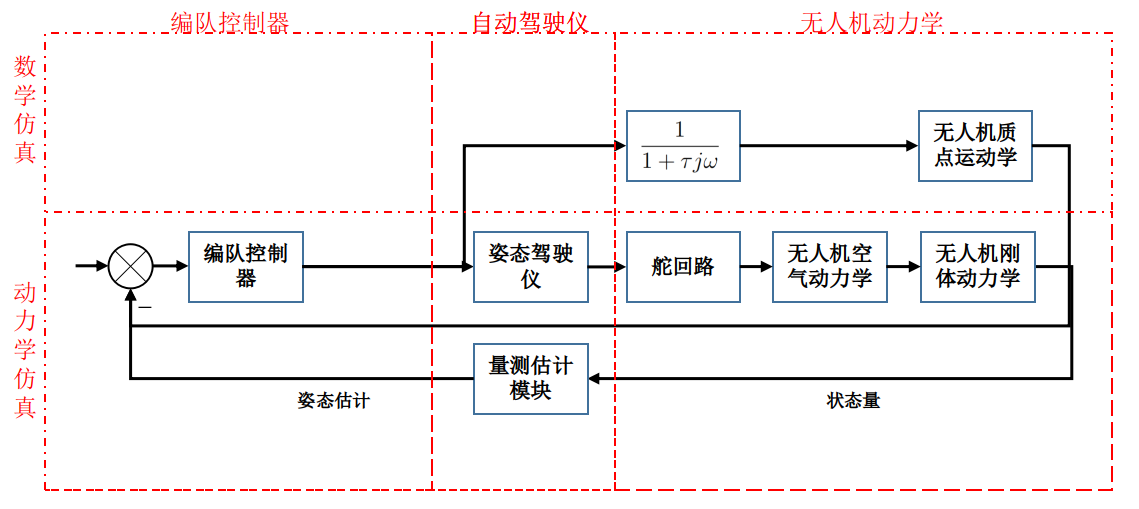
\includegraphics[width=0.85\textwidth]{figures/adds/contrust_sim}
    \caption{数学与动力学仿真实现方法}\label{fig:contrust_sim}
\end{figure}

在仿真结果上,动力学仿真相较于数学仿真,控制收敛时间明显加长,超调
量增大,稳态误差也有一定程度的增加,控制效果整体恶化。除去控制对象
本身的复杂性,动力学仿真环境产生的传感器噪声以及环境不确定性也使得控制
对象的复杂难度增加。
\section{本章小结}
本章主要分为三部分:第一部分着重介绍了本次设计所需要用到的仿真软件环境,详细介绍了Gazebo的软件架构,仿真机理以及仿真的相关特性。并通过ROS操作系统以及
MAVROS功能包搭建了与PX4内环进行数据交互的软件接口;之后结合Gazebo建立起了完整的编队控制器的无人机动力学仿真实验环境,
为后文的动力学仿真提供了相应的平台。
之后的主要工作是对于前文所设计的编队控制器进行响应的仿真:在第二部分,考虑无人机的质点运动模型,利用MATALB/Simulink等工具进行了
编队控制器的算法层面的数学仿真。在第三部分,利用前文中所介绍的Gazebo仿真环境进行编队控制器的动力学仿真,并整定了相关控制器的
参数,检验了控制器的稳定性,最后对两种仿真方式的关系做出了对比。
